% Options for packages loaded elsewhere
\PassOptionsToPackage{unicode}{hyperref}
\PassOptionsToPackage{hyphens}{url}
%
\documentclass[
]{article}
\usepackage{amsmath,amssymb}
\usepackage{iftex}
\ifPDFTeX
  \usepackage[T1]{fontenc}
  \usepackage[utf8]{inputenc}
  \usepackage{textcomp} % provide euro and other symbols
\else % if luatex or xetex
  \usepackage{unicode-math} % this also loads fontspec
  \defaultfontfeatures{Scale=MatchLowercase}
  \defaultfontfeatures[\rmfamily]{Ligatures=TeX,Scale=1}
\fi
\usepackage{lmodern}
\ifPDFTeX\else
  % xetex/luatex font selection
\fi
% Use upquote if available, for straight quotes in verbatim environments
\IfFileExists{upquote.sty}{\usepackage{upquote}}{}
\IfFileExists{microtype.sty}{% use microtype if available
  \usepackage[]{microtype}
  \UseMicrotypeSet[protrusion]{basicmath} % disable protrusion for tt fonts
}{}
\makeatletter
\@ifundefined{KOMAClassName}{% if non-KOMA class
  \IfFileExists{parskip.sty}{%
    \usepackage{parskip}
  }{% else
    \setlength{\parindent}{0pt}
    \setlength{\parskip}{6pt plus 2pt minus 1pt}}
}{% if KOMA class
  \KOMAoptions{parskip=half}}
\makeatother
\usepackage{xcolor}
\usepackage[margin=1in]{geometry}
\usepackage{graphicx}
\makeatletter
\def\maxwidth{\ifdim\Gin@nat@width>\linewidth\linewidth\else\Gin@nat@width\fi}
\def\maxheight{\ifdim\Gin@nat@height>\textheight\textheight\else\Gin@nat@height\fi}
\makeatother
% Scale images if necessary, so that they will not overflow the page
% margins by default, and it is still possible to overwrite the defaults
% using explicit options in \includegraphics[width, height, ...]{}
\setkeys{Gin}{width=\maxwidth,height=\maxheight,keepaspectratio}
% Set default figure placement to htbp
\makeatletter
\def\fps@figure{htbp}
\makeatother
\setlength{\emergencystretch}{3em} % prevent overfull lines
\providecommand{\tightlist}{%
  \setlength{\itemsep}{0pt}\setlength{\parskip}{0pt}}
\setcounter{secnumdepth}{-\maxdimen} % remove section numbering
  \usepackage{booktabs}
   \usepackage{longtable}
   \usepackage{array}
   \usepackage{multirow}
  \usepackage{wrapfig}
   \usepackage{colortbl}
   \usepackage{pdflscape}
   \usepackage{tabu}
   \usepackage{threeparttable}
   \usepackage{threeparttablex}
   \usepackage[normalem]{ulem}
   \usepackage{makecell}
   \usepackage{xcolor}
   \usepackage{placeins}
   \renewcommand{\topfraction}{.85}
   \renewcommand{\bottomfraction}{.7}
   \renewcommand{\textfraction}{.15}
   \renewcommand{\floatpagefraction}{.66}
   \setcounter{topnumber}{3}
   \setcounter{bottomnumber}{3}
   \setcounter{totalnumber}{4}
\usepackage{float}
\let\origtable\table
    \let\endorigtable\endtable
    \renewenvironment{table}[1][ht]{
      \expandafter\origtable\expandafter[H]
    }{
      \endorigtable
    }
\usepackage{booktabs}
\usepackage{longtable}
\usepackage{array}
\usepackage{multirow}
\usepackage{wrapfig}
\usepackage{float}
\usepackage{colortbl}
\usepackage{pdflscape}
\usepackage{tabu}
\usepackage{threeparttable}
\usepackage{threeparttablex}
\usepackage[normalem]{ulem}
\usepackage{makecell}
\usepackage{xcolor}
\ifLuaTeX
  \usepackage{selnolig}  % disable illegal ligatures
\fi
\IfFileExists{bookmark.sty}{\usepackage{bookmark}}{\usepackage{hyperref}}
\IfFileExists{xurl.sty}{\usepackage{xurl}}{} % add URL line breaks if available
\urlstyle{same}
\hypersetup{
  pdftitle={robustness},
  pdfauthor={Shadi},
  hidelinks,
  pdfcreator={LaTeX via pandoc}}

\title{robustness}
\author{Shadi}
\date{2023-07-06}

\begin{document}
\maketitle

\hypertarget{heterogeneous-treatment-effects-sun-abraham-2020}{%
\subsubsection{Heterogeneous Treatment Effects: Sun \& Abraham
(2020)}\label{heterogeneous-treatment-effects-sun-abraham-2020}}

Since 2018, there has been a growing body of literature examining the
validity of staggered Difference-in-Differences (DID) models and event
study designs. Noteworthy studies in this field include Goodman-Bacon
(2018), Callaway and Sant'anna (2020), de Chaisemartin and
D'aualtfoeuille (2020), Deshpande and Li (2019), Imai and Kim (2021),
and Baker et al.~(2021). Sun and Abraham (2021) highlight the challenges
that can arise when different treatment cohorts exhibit varying
treatment effects over time.

To address these concerns and assess the sensitivity of our event study
estimates to heterogeneous treatment effects, we adopt the
interaction-weighted (IW) event study estimator proposed by Sun and
Abraham (2021). This estimator is robust to variations in treatment
effects across cohorts. We estimate event study coefficients separately
for each group and outcome, and then aggregate these coefficients using
the fraction of the treated sample in each group as weights for the
relevant period. Importantly, the results of this analysis align with
our main findings.

We find no evidence of differential pre-trends, leading us to conclude
that our results are robust and not unduly influenced by variations in
treatment profiles across different cohorts.

\begin{center}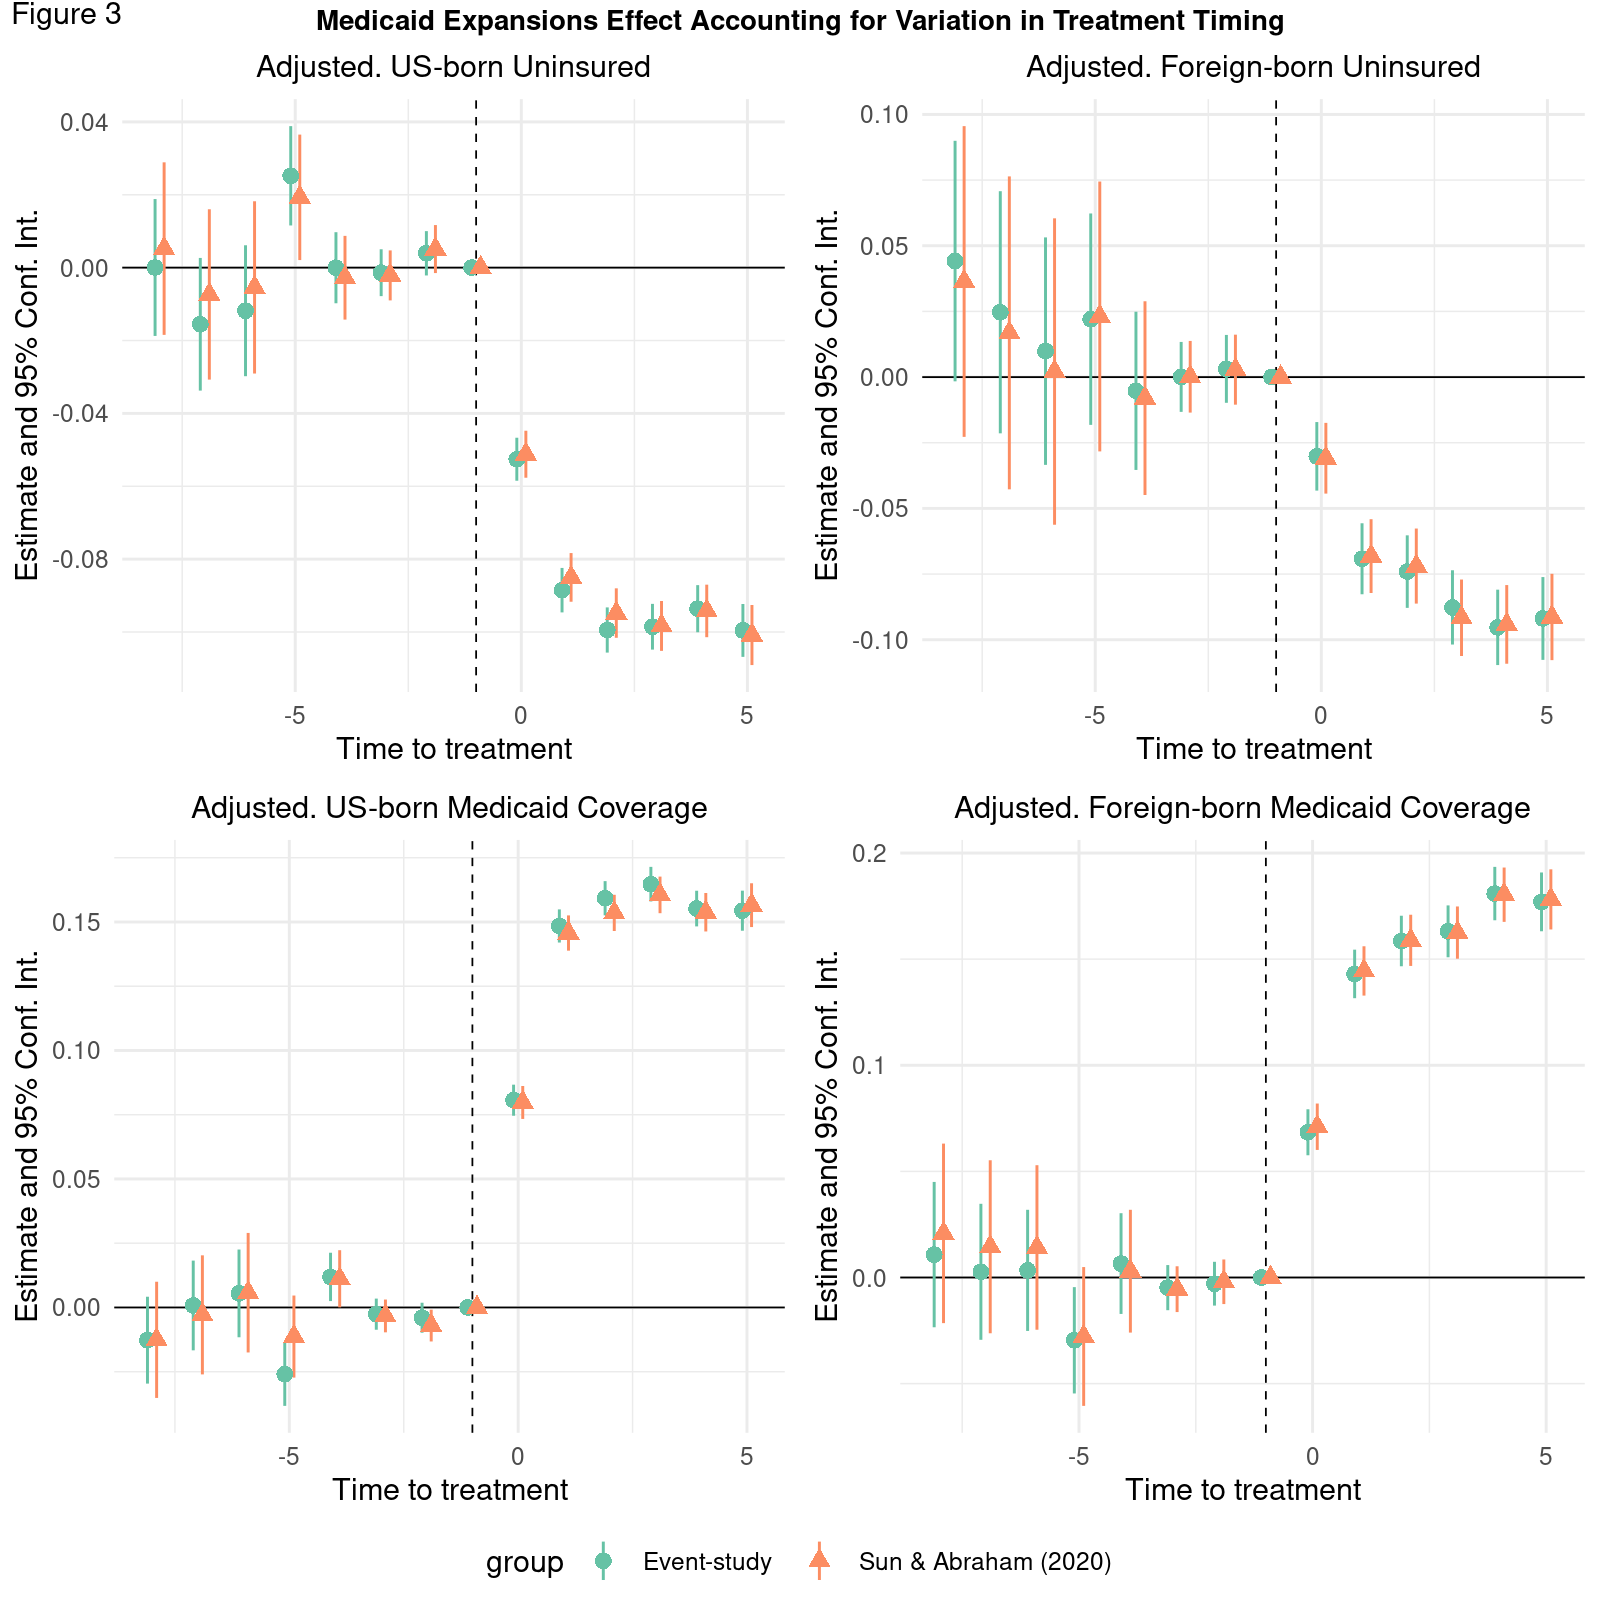
\includegraphics{/home/shadi/Projects/GitHub/medicaid-foreign-born/output/sun&abr-1} \end{center}

\hypertarget{difference-in-differences-estimate-bacon-decomposition-theorem}{%
\subsubsection{Difference-in-Differences Estimate: Bacon Decomposition
theorem}\label{difference-in-differences-estimate-bacon-decomposition-theorem}}

Employing Goodman-Bacon's (2018) methodology, we performed a
decomposition analysis utilizing two-way fixed effects
Difference-in-Differences (DID) estimators. This analysis provides
significant insights into the treatment effects and timing groups, as
outlined in Table 9.

\begin{table}

\caption{\label{tab:tab9}Bacon Decomposition}
\centering
\resizebox{\linewidth}{!}{
\begin{tabular}[t]{lll}
\toprule
Comparison & Coefficient & Weight\\
\midrule
\addlinespace[1em]
\multicolumn{3}{l}{\textbf{Uninsured}}\\
\hspace{1em}Earlier vs Later Treated & -0.09309 & 0.11871\\
\hspace{1em}Later vs Earlier Treated & -0.05521 & 0.08771\\
\hspace{1em}Treated vs Untreated & -0.08462 & 0.79358\\
\addlinespace[0.3em]
\multicolumn{3}{l}{\textbf{Medicaid}}\\
\hspace{1em}Earlier vs Later Treated & 0.14610 & 0.11871\\
\hspace{1em}Later vs Earlier Treated & 0.08782 & 0.08771\\
\hspace{1em}Treated vs Untreated & 0.14452 & 0.79358\\
\bottomrule
\end{tabular}}
\end{table}

The analysis involves comparing timing groups to units that never
received treatment, allowing us to evaluate the relative treatment
effects at different timings. Notably, a majority of the estimated
treatment effect can be attributed to the comparisons between treated
and untreated units, rather than comparisons between states with
different treatment times.

Furthermore, when we exclude the variation arising from comparisons of
states with different treatment times, the Difference-in-Differences
(DD) estimate remains highly consistent with the main DD estimate. In
simpler terms, the magnitude of the treatment effect produced by the
2014 wave is comparable to the effects observed in subsequent waves.
This robustness analysis strengthens our findings and affirms the
reliability of the estimated treatment effect.

\begin{center}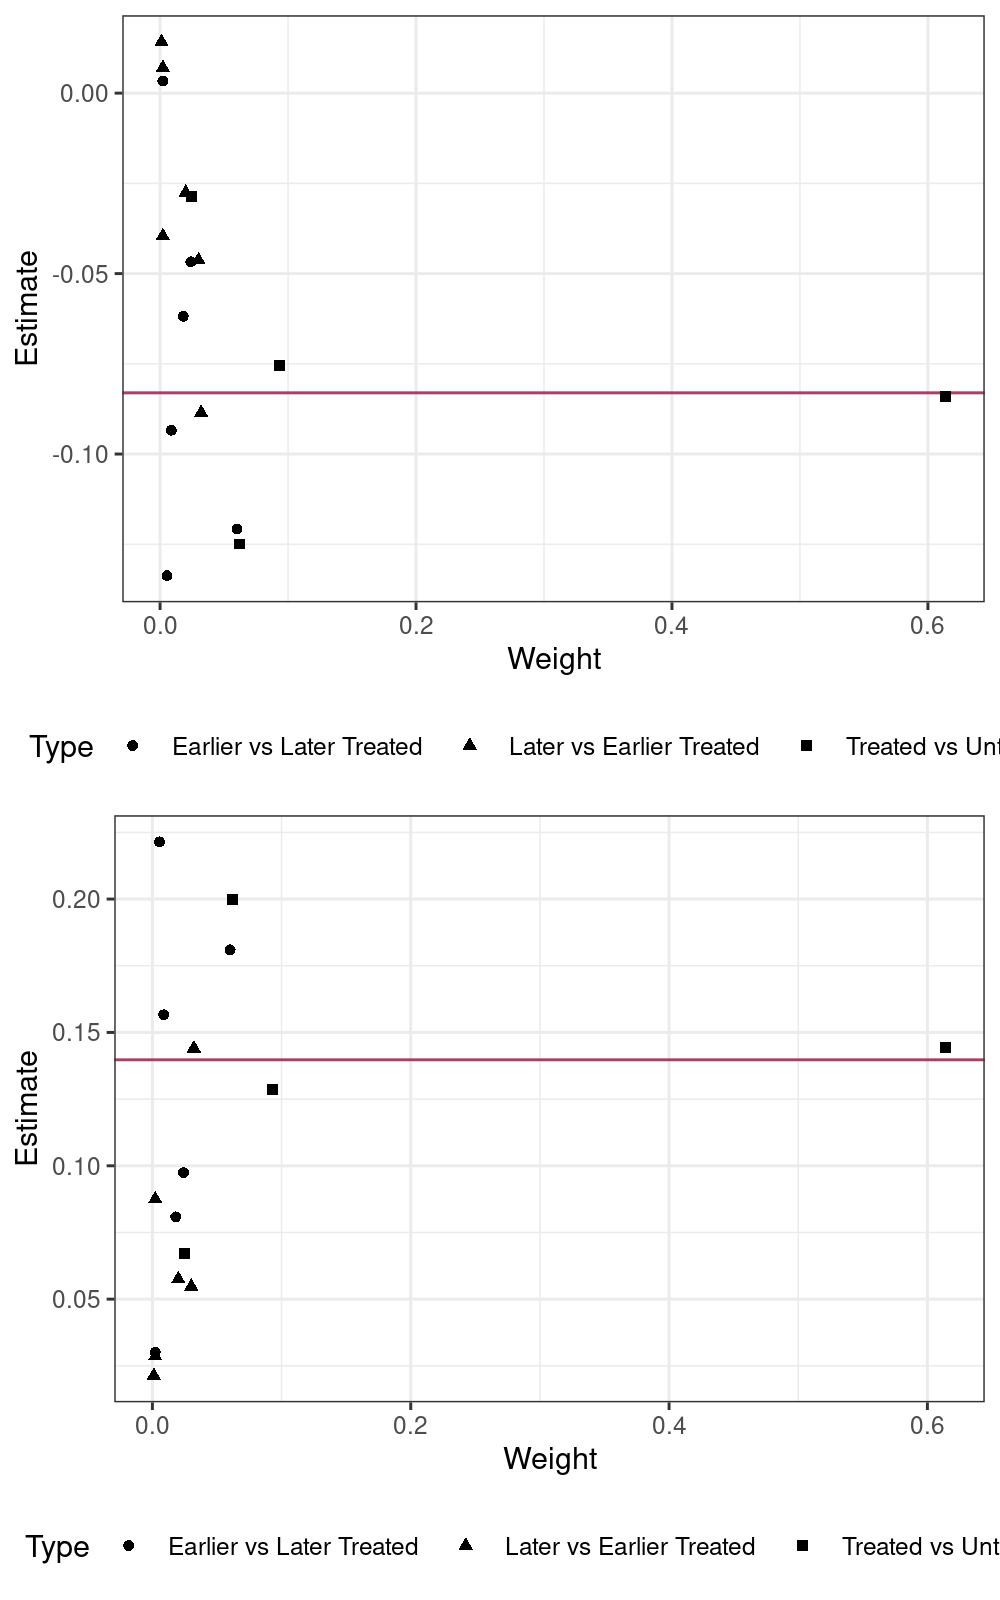
\includegraphics{/home/shadi/Projects/GitHub/medicaid-foreign-born/output/plotbac-1} \end{center}

Figure 4 provides support for this finding by presenting the 2 × 2 DD
estimates and associated weights derived from the conventional two-way
fixed effect model. Panel (a) illustrates the estimates for the
Uninsured group, while panel (b) exhibits the estimates for Medicaid
coverage.

\end{document}
